\documentclass{article}
\usepackage[preprint]{neurips_2022}
\usepackage{amsfonts}       % blackboard math symbols
\usepackage{amsmath}
\usepackage{booktabs}       % professional-quality tables
\usepackage{float}
\usepackage[T1]{fontenc}    % use 8-bit T1 fonts
\usepackage{graphicx}
\usepackage{hyperref}       % hyperlinks
\usepackage[utf8]{inputenc} % allow utf-8 input
\usepackage{microtype}      % microtypography
\usepackage{wrapfig}
\usepackage{xcolor}         % colors
\title{Bilingual Offline Transcriptions}
\author{
  Yizhen Yu \\
  Carnegie Mellon University\\
  Pittsburgh, PA 15213 \\
  \texttt{yizheny@andrew.cmu.edu} \\\And
  Henry Wu \\
  Carnegie Mellon University \\
  Pittsburgh, PA 15213 \\
  \texttt{zhenyuW@andrew.cmu.edu}
}
\begin{document}
  \maketitle
  \begin{abstract}
    This project examines different approaches to implementing and improving ASR for input in more than one language, with a focus on improving accuracy with low hardware and training time requirements. This is a task that has wide applicability in fields that deal with bilingual and multilingual content, such as transcripts of video interviews and translation software for live conversations. We found that a successful strategy to improve both training speed and evaluated error rate is to introduce language markers---whether in speech or text---to the training samples.
  \end{abstract}
  \section{Introduction [Yizhen Yu]}
  \subsection{Advancements in Automatic Speech Recognition}
  \textbf{Automatic speech recognition (ASR)}, the process of transforming human speech into readable text, has long been an area of popular research in machine learning. A number of such end-to-end model architectures, including RNN-\footnote{\cite{Chan}}, transformer-\footnote{\cite{Vaswani}}, and conformer-based\footnote{\cite{Gulati}} methods, have steadily improved performance on ASR tasks, largely displacing traditional HMM/GMM architectures that learn explicit acoustic, lexicon, and language models and require domain knowledge.

  A state-of-the-art architecture by \cite{Kim} on which we base our project is a hybrid model combining connectionist temporal classification (CTC), a concept originally proposed in RNN models, and attention, a core principle of transformers and conformers. However, these methods have largely focused on training and running on a single language---usually English---while situations that include bilingual speech are largely overlooked. In this project, we explore a selection of strategies to investigate the ease and effectiveness with which we may introduce bilingual support.
  \subsection{The Need for Multilingual Transcription}
  The ability to recognize and transcribe speech in more than one language can be applied to many problems that remain unaddressed today. A common phenomenon in conversations involving bilingual individuals is \textbf{code switching}, in which a speaker changes languages within a single unit of speech\footnote{\url{https://en.wikipedia.org/wiki/Code-switching}}. This can happen at a number of different levels---among different sentences in a conversation, among words or phrases in a sentence, and even among parts of a single word.

  This project will focus on the first two levels, training end-to-end networks to transcribe human voice clips containing phrases or complete sentences in one or two target languages. (This task is different from that of \textbf{speech translation}, in which the input is in one language and the output is in another.) This is a problem that is noticeably underserved in both literature and implementation. Even mature speech transcription services such as YouTube's automatic captioning\footnote{\url{https://support.google.com/youtube/answer/6373554?hl=en}} fail to handle well-separated speech in two languages, such as in videos of foreign-language interviews.

  The goal of this project is to demonstrate, experiment with, and evaluate the introduction of bilingual speech into different ASR model configurations, with a focus on improving accuracy with low hardware and training time requirements.
  \section{Data [Yizhen Yu]} \label{data}
  The input of the trained models take the form of audio clips of human speech in one or two languages, each a few seconds long and normalized to 16 kHz FLAC. (This may sound low to people who are used to sampling rates for music, but it's actually twice the standard telephony sampling rate of 8 kHz\footnote{\url{https://www.phonetik.uni-muenchen.de/forschung/BITS/TP1/Cookbook/node61.html}} and well-suited to voice data.) The output is a unicase plain-text transcription of what was said, including spaces and punctuation. Some preprocessing is done to sanitize and augment the dataset by excluding clips that are very short (less than 0.1 seconds long) and very long (more than 20 seconds long) and then duplicating the remaining samples at $0.9 \times$, $1.0 \times$, and $1.1 \times$ playback speeds.

  The speech clips and text transcriptions of the training, validation, and test datasets come from Mozilla's Common Voice 11\footnote{\url{https://commonvoice.mozilla.org/en/datasets}}, a crowdsourced collection of over 24 thousand hours of audio clips in dozens of languages. In particular, the Lithuanian (LT) and Slovak (SK) collections were selected for due to their small size (19 validated hours each), their relative completeness, and the fact that they share the Latin script, which reduces the output character space of the model. A further eight hours of Latvian data from the same source is used for augmentation in an experiments (see Section \ref{experiment-latvian-augmentation}).

  For sentence-level code switching, we simply run the model on clips from a randomly selected language. Due to the lack of bilingual speech datasets with validated transcriptions, we simulate phrase- and word-level code switching by simply concatenating clips of SK and LT speech, then concatenating their corresponding validated transcriptions separated by a space, simulating bilingual LT/SK speakers. There are some drawbacks to this approach:
  \begin{itemize}
    \item the transition between clips may be abrupt and unlike a natural interval between phrases
    \item the concatenated samples may be of very different character or grammatical function
  \end{itemize}
  These effects imply that the error rates we see on these concatenated samples are likely to exceed those of real speech exhibiting code switching, since such a sample would have a more consistent structure and be more cohesive in meaning.
  \section{Background [Yizhen Yu]}
  \subsection{Dataset Configurations}
  We consider three different basic arrangements of the dataset:
  \begin{itemize}
    \item models trained on a single language of interest, Slovak (``Single-Language'')
    \item models trained on samples taken randomly from both languages of interest (``Combined'')
    \item models trained on samples constructed by concatenating samples from both languages of interest, as described in Section \ref{data} (``Concatenated'')
  \end{itemize}
  Since the Concatenated dataset is a little trickier to work with than the Combined dataset, our experiments were conducted and tuned on the Combined dataset, with the learnings applied to the Concatenated dataset for evaluation.
  \subsection{Previous Results} \label{previous-results}
  Previous testing (described in the Midway Report) indicate that the default conformer--transformer configuration provided by ESPnet performs very well out of the box on the Combined dataset. However, this is likely due to the architecture, being complex enough to handle a larger language model, treating the combination of the relatively small Lithuanian and Slovak datasets as a single language of middling size.
  \begin{wrapfigure}{r}{0.5\textwidth}
    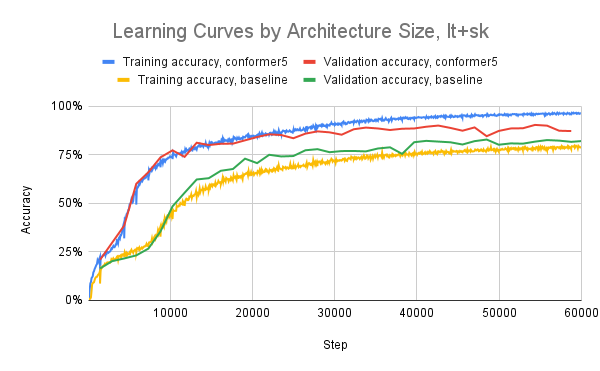
\includegraphics[width=0.5\textwidth]{images/learning-architecture}
    \caption{Learning curves of the conformer5 (large) and baseline (small) models.}
  \end{wrapfigure}
  Such a characterization would also explain the moderate amount of overfitting observed in the preliminary results, with validation accuracy levelling off well before training accuracy did. This is one of the reasons we made an effort to reduce model complexity before further experimentation, as described in Section \ref{baseline-model-selection}.

  Interestingly, the validation accuracy of the baseline model actually \emph{exceeds} its training accuracy. This is likely due to an uneven split in the relatively small dataset, where more difficult samples ended up in the training data.

  See Section \ref{metrics} for a detailed description of the accuracy metric depicted.
  \section{Related Work [Yizhen Yu]} \label{related-work}
  Three papers are notable for their influence as prior work while we developed this project.

  \cite{Yilmaz} investigates bilingual speech recognition between Dutch and Frisian, a minority language spoken in the North of Netherlands. As the two languages are influenced by each other, code-switching is common among speakers. The authors develop DNNs to perform ASR by two different methods: with distinct sets of phones\footnote{\url{https://en.wikipedia.org/wiki/Phone_(phonetics)}} as targets for each language (``language-dependent'') and with a shared set of phones as targets for both (``language-independent''). In terms of problem setup, this is the paper we found most directly related to our project, although we aim to demonstrate an approach using an end-to-end model that does not require explicit acoustic modelling as used in the paper.

  \cite{Liu} develops multilingual machine translation on a wider variety of languages using the mBART model, with a sequence-to-sequence auto-encoder trained on large monolingual corpora in many languages and a transformer decoder, comparing performance on models pretrained on different numbers of languages. This architecture is more similar to ours, with the now-standard attention-based encoder--decoder setup. Note that although this paper deals with machine \emph{translation} rather than transcription, it's notable for two innovations, both of we experiment with:
  \begin{itemize}
    \item distinguishing languages by labelling sentences with a language marker
    \item training on languages beyond those of interest (so that the training dataset includes more languages than the test dataset)
  \end{itemize}
  The core architecture used in this project is based on \cite{Kim}'s hybrid CTC/attention model using modern conformer and transformer units (implemented as part of ESPnet). See Section \ref{architecture} for a detailed description of how and why it applies to our project.
  \section{Methods [Yizhen Yu]}
  \subsection{Baseline Model Selection} \label{baseline-model-selection}
  Due to the feasibility of repeatedly training ASR models on dozens of hours of speech using the limited hardware available, we first endeavored to find a small model configuration that was still complex enough to converge on our tasks. We achieved this by starting with the default conformer--transformer configuration provided by ESPnet and tuning a few hyperparameters to satisfy the following requirements with our Combined dataset:
  \begin{enumerate}
    \item Validation accuracy (defined in Section \ref{metrics}) needs to level off after training for at most 5 hours on a single GTX 1070. This is a visual indication we used to determine that the model was capable of converging.
    \item Word and character error rates need to settle within a reasonable range. This is a very subjective requirement, but the goal is to be able to evaluate models that successfully learned to perform ASR while leaving room for improvement in experimentation.
    \item Little or no overfitting may be present. Since we pose the problem as a challenge to perform well with low resource requirements, overfitting would indicate that we had more room to simplify the architecture and reduce overparameterization
  \end{enumerate}
  \begin{wrapfigure}{r}{0.5\textwidth}
    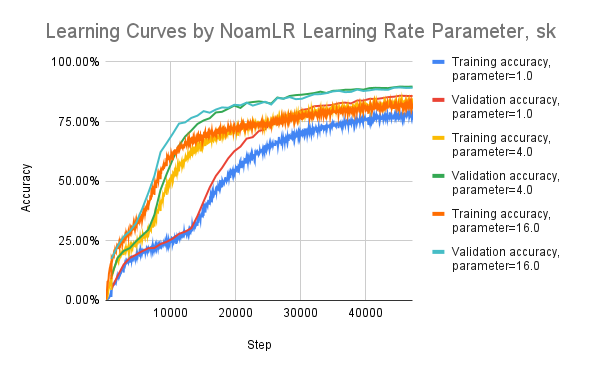
\includegraphics[width=0.5\textwidth]{images/learning-learning-rate}
    \caption{Learning curves of the baseline (small) models on Slovak with various learning rate parameters.}
  \end{wrapfigure}
  Some broad architecture hyperparameters were adopted from the original transformer paper,\footnote{\cite{Vaswani}} in particular the reduction of the number of attention units in the encoder and decoder to 6. Due to its impact on convergence during training and its sensitivity to architecture size, we tuned learning rate with a parameter sweep on the Single-Language (Slovak) dataset.

  A learning rate parameter of 4.0 was chosen for our baseline due to its superior performance. Note that this is the parameter used for NoamLR, a learning rate scheduler first proposed by \cite{Vaswani}, not the actual learning rate. The initial learning rate is $\frac{\mathrm{learning\ rate\ parameter}}{\sqrt{\mathrm{model\ size}} \cdot \sqrt{\mathrm{warmup\ steps}}} = \frac{4}{\sqrt{256} \cdot \sqrt{25000}} = 10^{-3}$, where the denominator contains two hyperparameters that were not tuned.
  \subsection{Network Input} \label{network-input}
  The basic problem of ASR is to learn some $p(W \mid X)$ where $X$ is a sequence of speech features and $W$ is a sequence of words in the target language. As a speech-to-text model, inference can be expressed as $\hat{W} = \hat{f}(X)$ where $\hat{f}$ is the learned inference function.

  In the ESPnet model, this problem is simplified by instead learning $p(T \mid X)$ where $T$ is a token sequence (see \ref{metrics}). As such, the samples used for training (paired speech clips and text transcriptions) are first preprocessed by reading the single-channel waveform at 16 KHz (using \texttt{soundfile.read}\footnote{\url{https://pysoundfile.readthedocs.io/en/latest/}}) into a vector normalized to $[-1, 1]^*$ (a sequence of arbitrary length of real numbers in the interval) and tokenizing the text into a vector of token IDs (a sequence of nonnegative integers, padded to length 64 with the special value $-1$).

  Each token ID represents a key in a token map specific to the dataset. In our case, the token maps are precomputed over the dataset as the replacement tables generated by a byte-pair encoding (BPE) algorithm.\footnote{\url{https://huggingface.co/course/chapter6/5?fw=pt}}. Special token IDs are reserved for marking the beginning and end of the sequence, the CTC \texttt{<blank>} as defined in Section \ref{architecture}, and other unprinted information; it is also adapted for language markers in Section \ref{experiments}.
  \subsection{Architecture} \label{architecture}
  \begin{table}
    \begin{center}
      \begin{tabular}{lrr}
        \toprule
        Parameter                           & Baseline & confromer5 \\\midrule
        Conformer layers (encoder)          & 6        & 12 \\
        Transformer layers (decoder)        & 6        & 6 \\
        Encoder output / decoder input size & 64       & 256 \\
        Encoder linear layer width          & 2048     & 256 \\
        Decoder linear layer width          & 2048     & 256 \\\bottomrule
      \end{tabular}
    \end{center}
    \caption{Architecture hyperparameters for our baseline model as well as the default conformer5 model provided by ESPnet.}
    \label{table-architecture-hyperparameters}
  \end{table}
  The core architecture used in this project is based on \cite{Kim}, an attention-based end-to-end ASR model using CTC loss as a regularizer to encourage representations of the speech/text samples to remain in the right order. The complete architecture is a configuration of ESPnet's basic model.

  The overall architecture consists of a conformer encoder and transformer decoder, each with six (parallel) layers. After hyperparameter tuning, we configured each encoder and decoder layer with 256-wide fully-connected layers and 64-wide attention layers and trained them with a dropout rate of 0.1. Complete parameter details in ESPnet configuration format can be found in the attached \textit{train\_asr\_conformer5\_linear-units-256-output-64-num-blocks-6.yaml}. For baseline comparisons, we run some tests on the full conformer5 model as provided by ESPnet. See Table \ref{table-architecture-hyperparameters} for a summary.
  \begin{wrapfigure}{l}{0.4\textwidth}
    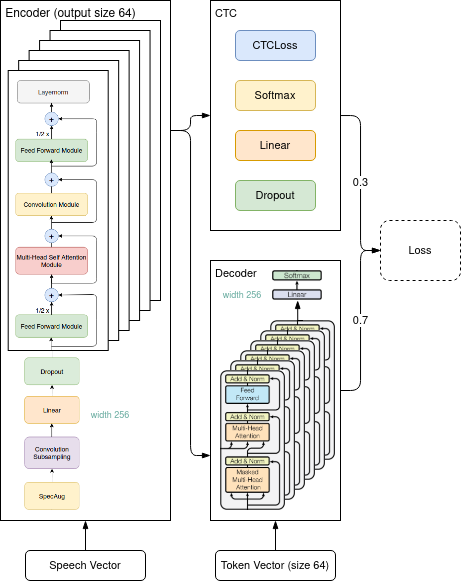
\includegraphics[width=0.4\textwidth]{images/architecture}
    \caption{Basic architecture of the ASR model. Notable differences from the default ESPnet conformer5 model are noted in green. See \textit{train\_asr\_conformer5\_linear-units-256-output-64-num-blocks-6.yaml} for more hyperparameters.}
  \end{wrapfigure}
  In parallel with the decoder is a CTC module, which does not contribute to the output transcript in inference but does contribute to training loss. In principle, the architecture is designed to take advantage of both the contextual information retained by the attention modules and the sequence enforcement by the CTC module. (The latter effect is useful here but not in \cite{Liu}, because ASR generally expects output order to roughly align to input order, which is not generally the case in machine translation.)

  The loss function is a weighted average
  $$
    \mathrm{loss} = \lambda \mathrm{loss}_{\mathrm{CTC}} + \left(1 - \lambda\right) \mathrm{loss}_{\mathrm{attention}}
  $$
  of the CTC and attention losses, which correspond to the CTC and attention objectives
  \begin{align*}
    p(T \mid X) &= p(T \mid Z) \, p(Z \mid X)
                 = \frac{p(Z \mid T) \, p(T)}{p(Z)} \, p(Z \mid X) \\
                &= p(Z \mid X) \prod_{i = 1}^n p \left(z_i \mid z_1, \cdots, z_{i - 1}, T\right) \, \frac{p(T)}{p(Z)} \\
                &\approx p(Z \mid X) \prod_{i = 1}^n p \left(z_i \mid z_{i - 1}, T\right) \, \frac{p(T)}{p(Z)}
  \end{align*}
  and
  $$
    p(T \mid X) = \prod_{i = 1}^l p \left(t_i \mid t_1, \cdots, t_{i - 1}, X\right)
  $$
  where $Z = \left\{z_1, \cdots, z_n\right\}$ assuming conditional independence on the $z_i$s is the token sequence augmented by interleaving the special symbol \texttt{<blank>} and $p \left(z_i \mid z_{i - 1}, T\right)$ is a simple binary function as defined in \cite{Kim}.

  Note that the CTC loss (using PyTorch's implementation\footnote{\url{https://pytorch.org/docs/stable/generated/torch.nn.CTCLoss.html}}) is carried through the encoder and CTC module, while the attention loss (a mean of token ID equalities between the decoded output and the true value) is carried through the encoder and decoder.

  Inference is conducted through a beam search for candidate transcriptions. The main difference between this model and the one in \cite{Kim} is the use of token IDs rather than characters.
  \subsection{Experiments} \label{experiments}
  \subsubsection{Language markers}
  Four different approaches to language markers were implemented: single-byte speech markers, audio-clip speech markers, explicit text markers, and tokenized text markers.  Motivations for these approaches are discussed in \ref{results}.
  \begin{enumerate}
    \item \textbf{Single-byte speech marker:} We inject a single byte, either $+1$ for LT or $-1$ for SK, at the beginning of the normalized speech input vector before passing it into the encoder.
    \item \textbf{Audio-clip speech marker:} Instead of a single byte, we concatenate a one-second clip of a male voice saying ``Lithuanian'' or ``Slovak'' to the beginning of the sample speech input before they are converted to waveforms and normalized to an input vector. The clips used in our experiments are provided as \textit{lt.mp3} and \textit{sk.mp3}.
    \item \textbf{Explicit text marker:} Similar to the approach taken by \cite{Liu}, two nonprintable tokens, \texttt{<lt>} and \texttt{<sk>}, are provided as explicit additions during the token map generation phase (see Section \ref{network-input}). During preprocessing, the IDs of these tokens are injected at the beginning of the token ID vector before it is passed to the decoder.
    \item \textbf{Tokenized text marker:} This is similar to the above, but we modify the sample data itself by prepending the text \texttt{<lt>} and \texttt{<sk>} to samples in the dataset, so that we do not need to modify the proprocessing stage. We also explicitly add them to the token map as described above.

    The initial goal was for the token map generation to automatically register these as tokens, but it did not do so and we were unable to quickly debug the reason. This is left as potential future work.
    \item \textbf{Both speech and text:} Both audio-clip speech markers and tokenized text markers are applied to the dataset.
  \end{enumerate}
  \subsubsection{Augmentation With Latvian} \label{experiment-latvian-augmentation}
  As seen in \cite{Liu}, training on languages not in the test set may be beneficial as a form of data augmentation. We attempt this by incorporating eight hours of samples in Latvian, a language closely related to Lithuanian. Mid-training evaluations over training and validation datasets are done over all three languages, while final error calculation over the test dataset is done over Lithuanian and Slovak only.
  \subsubsection{Other Experiments: Transformer Architecture}
  We also implemented a transformer experiment using the same architecture as the baseline conformer, but with the conformer layers in the encoder replaced by transformer layers. Fatal errors were encountered during training which unfortunately could not be addressed due to time constraints.
  \section{Results [Yizhen Yu]} \label{results}
  \subsection{Metrics} \label{metrics}
  ESPnet provides utilities for calculating sentence (SER), word (WER), token (TER), and character error rates (CER) on ASR output as part of model evaluation. In our case, tokens are subword divisions computed by BPE; see Section \ref{network-input} for more details.

  The accuracy values reported during the training stage are by token. (The loss functions is a weighted average of the TER and the CTC loss, which is a metric on alignments in two sequences, expressed as a sum of probabilities, as described in Section \ref{architecture}.) For convenience, this token-level accuracy metric (the percentage of tokens in the decoder output that match the corresponding tokens in the validated text) is used for all plots of learning curves, while the more standard WER metric is reported at the end of training for each experiment. Note that in general, we would expect WER to be at least as large as TER, since for a word to be correct its subword divisions must match as well.
  \subsection{Baseline Comparisons} \label{results-baseline-comparisons}
  First, it's important to note that the comprehensiveness of a dataset is critical in determining the success of any model trained on it. To sanity-check the validity of our error rate calculations, we compare the results for three datasets trained on the full conformer5 model of varying sizes. There is some apparent correlation, which justifies the high error rates we encounter in our results in general, as they all come from a relativvely small dataset.
  \begin{table}
    \begin{center}
      \begin{tabular}{lrrrr}
        \toprule
        Dataset trained on conformer5                                                                       & Dataset size & WER    & CER    & TER \\\midrule
        Assamese                                                                                            & 0.3 hours    & 100\%  & 100\%  & 100\% \\
        Combined                                                                                            & 38 hours     & 45.3\% & 13.3\% & 19.1\% \\
        Italian (ESPnet)\footnote{\url{https://github.com/espnet/espnet/tree/master/egs2/commonvoice/asr1}} & 131 hours    & 16.1\% & 4.4\%  & 5.3\% \\
        Polish (ESPnet)\footnote{\url{https://github.com/espnet/espnet/tree/master/egs2/commonvoice/asr1}}  & 105 hours    & 2.6\%  & 1.2\%  & 1.1\% \\
        Russian (ESPnet)\footnote{\url{https://github.com/espnet/espnet/tree/master/egs2/commonvoice/asr1}} & 106 hours    & 7.9\%  & 2.1\%  & 2.8\% \\\bottomrule
      \end{tabular}
    \end{center}
    \caption{Comparison of error rates on datasets of varying sizes trained on conformer5. ``Combined'' denotes our Combined dataset as defined in Section \ref{data}. The bottom three results are published values.}
    \label{table-conformer5-results}
  \end{table}
  We then compare the baseline results for the individual-language, Combined, and Concatenated datasets. As expected, both of the latter datasets have higher error rates but are comparable to each other, indicating that they were learned together as one language with a deeper orthography than both\footnote{\url{https://en.wikipedia.org/wiki/Orthographic_depth}}:
  \begin{table}
    \begin{center}
      \begin{tabular}{lrrrr}
        \toprule
        Dataset trained on baseline model & Dataset size & WER    & CER    & TER \\\midrule
        Lithuanian                        & 19 hours     & 66.2\% & 19.9\% & 32.1\% \\
        Slovak                            & 19 hours     & 57.7\% & 18.4\% & 26.0\% \\
        Combined                          & 38 hours     & 75.7\% & 24.5\% & 35.2\% \\
        Concatenated                      & 38 hours     & 73.5\% & 22.9\% & 33.9\% \\\bottomrule
      \end{tabular}
    \end{center}
    \caption{Comparison of error rates on datasets of varying sizes trained on the baseline model.}
    \label{table-baseline-results}
  \end{table}
  \subsection{Experiment results}
  \begin{table}
    \begin{center}
      \begin{tabular}{lrrr}
        \toprule
        Experiment     & WER    & CER    & TER \\\midrule
        Baseline       & 75.7\% & 24.5\% & 35.2\% \\
        Single byte    & 75.6\% & 24.9\% & 35.6\% \\
        Audio clip     & 64.8\% & 18.4\% & 27.2\% \\
        Explicit text  & 90.3\% & 35.5\% & 40.6\% \\
        Tokenized text & 74.7\% & 22.8\% & 33.3\% \\
        With Latvian   & 94.9\% & 64.0\% & 62.1\% \\\bottomrule
      \end{tabular}
      \begin{tabular}{lrrr}
        \toprule
        Experiment      & WER    & CER    & TER \\\midrule
        Concatenated    & 73.5\% & 22.9\% & 33.9\% \\
        Audio clip      & 100\%  & 81.2\% & 96.4\% \\
        Tokenized text  & 69.5\% & 18.9\% & 28.9\% \\
        Speech and text & 68.5\% & 18.0\% & 27.8\% \\\bottomrule
      \end{tabular}
    \end{center}
    \caption{Comparison of error rates on datasets of varying sizes trained on the baseline model.}
  \end{table}
  The single-byte speech marker approach produced no noticeable change in error rates at all. This is likely because a single byte does not conform well to the form of features in the rest of the clip, and is of negligible size when compared to the full input vector.

  The audio-clip speech marker approach was motivated as a way to address the above. Theoretically, the encoder should be able to learn to transform the characteristic marker clip features as a dimension in the output embedding as passed to the decoder. We see a significant improvement over baseline in the Combined dataset but not the Concatenated.

  The best single approach was to inject language marker tokens into the input text, reducing all three error rate metrics on both datasets. Combining it with the audio-clip speech marker yielded slightly better results, but not by much.

  The single-byte speech marker, explicit text marker, and augmentation with Latvian experiments were excluded from the Concatenated dataset due to poor results on the Combined dataset.

  Surprisingly, training a three-language model with Latvian and evaluating it on LT and SK yielded terrible results. A brief perusal of the output transcripts indicates this this is likely not a bug in evaluation but an actual issue with the generated transcripts.
  \section{Discussion and Analysis [Yizhen Yu]}
  \subsection{Conclusion}
  We propose through this project an approach to training an ASR system that supports speech in more than one language. This is the problem area we set out to investigate as it has any applications underserved by existing models. Taking inspiration from \cite{Liu}'s approach to combining machine-translation models for multiple languages into a single model, we find that many of the same tricks can be applied to multilingual ASR tasks as well. In particular, introducing language markers to signal the introduction of one of the languages supported by a model was found to provide a significant boost to transcription accuracy.

  At its core, these techniques are a way to build into the common model an awareness of the distinct languages in the dataset. As seen in Section \ref{previous-results} and confirmed in Section \ref{results-baseline-comparisons}, it's likely the case that naively training a single model on samples from multiple languages, whether those samples are separated by language (as in the Combined dataset) or combined (as in the Concatenated dataset), causes the model treat the complete dataset as a single language with a deep orthography. The fact that adding explicit markers in either the speech or the text of a sample causes a significant decrease in error rate implies that the additional information is being incorporated into the model's representation of the sample---in effect, that it should be treated as one language or another.
  \subsection{Limitations}
  A few caveats may be noted about our results and conclusions.

  The first is a matter of dataset size. Commonvoice Lithuanian and Slovak are not particularly large datasets when compared to those used by state-of-the-art ASR engines, such as Commonvoice English and Spanish. It may be difficult to extrapolate these conclusions to a more comprehensive model trained on better data.

  The second is the fact that we have introduced more data into the system than would be needed for a classic ASR task. This is particularly the case with the audio-clip speech markers, since the markers were applied during inference as well. As such, we should treat this approach as a form of \emph{enhanced} ASR.
  \subsection{Future Work}
  Much further work can be done for the development of multilingual ASR systems. A few particular questions can be drawn from the results of these experiments:
  \begin{enumerate}
    \item Since we conclude that language markers are useful for training multilingual ASR systems, would it be possible to augment real recordings of bilingual speech containing code switching by automatically detecting and marking languages in them? An approach like \cite{Yilmaz} may be useful to integrate into the training of such a system. This would allow for the training of data more relevant to the problem statement.
    \item Lithuanian and Slovak both belong to the Balto-Slavic branch of the Indo-European language family, but they are not particularly similar to one another. Does language similarity affect the ability of a model to distinguish between them?
    \item We found that incorporating Latvian data \emph{decreases} model quality. Further investigation would be useful in determining whether this is simply the result of the larger representation space that the model now has to learn, if the dataset is of inferior quality compared to the languages of interest, or if there is some fundamentally detrimental interaction between the Latvian data and some other portion of our dataset, such as the Lithuanian data.
  \end{enumerate}
  \newpage
  \bibliographystyle{plainnat}
  \bibliography{references}
  \section*{Video presentation available at \url{https://drive.google.com/file/d/19-r9yDjjO8qEgvQIJ0XGeCIfWoi-Wj8-/view?usp=sharing}}
  \section*{Code available at \url{https://fishbotwilleatyou.com/10701/}}
\end{document}
